\chapter{Segunda Iteración}

Como se explica en el la subsección \ref{metodologiadedesarrollo}, en la que se expone la metodología de desarrollo utilizada para el proyecto, este sufre de tres grandes iteraciones para su completitud. En esta sección se explican los detalles implementados en la segunda iteración, es decir, la generación de un mejor diseño de la aplicación, nuevas interfaces, refactorización de clases y código replicado, así como mejoras gráficas visuales dentro de la aplicación, incluyendo referencias a la sección \ref{primeraiteracion}, explicando los cambios en diseño y comportamiento.

\section{Arquitectura del Proyecto}
\label{it2arquitectura}

La arquitectura del proyecto ha cambiado radicalmente desde la primera iteración, en la que estaba centrada en cómo se debería tratar el documento de especificación de juego, incluido dentro del paquete del juego, en forma de XML para que, cada elemento fuese lo más dinámico posible y sostenible. A su vez, estaba centrada en la clase Game, y existían multitud de clases, llamadas clases de utilidad, que contenían funcionalidad que debía ser accesible a través de una clase controladora de nivel superior.

En esta arquitectura encontramos tres paquetes importantes que engloban la funcionalidad necesaria para la ejecución del proyecto. Están representados en la figura \ref{arquitecturait2} Estos tres paquetes son:

\begin{itemize}
	\item \textbf{Core}: \textit{Core} contiene el núcleo de eAdventure portado a Unity. Este paquete está formado, a su vez, por varios subpaquetes. El primero de ellos es \textit{DataModel}, donde se encuentra todo el modelo de datos portado de eAdventure a Unity, siendo completamente fiel a la implementación realizada en Java, y soportando todas las funcionalidades que se soportaban en dicho editor. El segundo de ellos es \textit{Loader}, donde está contenido el nucleo de lectura y carga del fichero XML de especificación del juego. Este \textit{Loader}, recibe un XML y genera un objeto \textit{AdventureData} que contiene todos los datos del juego. Por último, dentro de \textit{Core} encontramos un paquete \textit{Auxiliar} con clases útiles para este modelo de datos.
	
	\item \textbf{RAGETracker}: que contiene los elementos necesarios para generar un registro de actividad de juego del usuario y comunicarse con RAGE a través de Unity. RAGE se encarga de realizar tareas de evaluación y \textit{Learning Analytics} mediante el análisis de las trazas producidas por el alumno mientras juega. Esto permite al profesor que esté utilizando un juego producido con uAdventure, que se beneficie de las ventajas de RAGE, pudiendo reforzar aquellos alumnos que estén teniendo un desarrollo insuficiente o anormal en el juego.
	
	\item \textbf{Runner}: que se encarga de la transformación desde la especificación una ruta donde hay un juego descomprimido, hasta la generación de un entorno gráfico interactivo que permite al usuario jugar al juego. Contiene 3 subpaquetes que se encargan de diferentes tareas. En primer lugar, el paquete ResourceManager, que se encarga de la carga transparente de recursos, ya sean imágenes, videos, botones, cursores, u otros elementos multimedia. En segundo lugar, el paquete Appearance, que se encarga de mejorar la visualización, mediante diferentes formas de mostrar burbujas de diálogo, o mediante el uso de Shaders. Por último, el paquete \textit{GameLogic and Representation} que se encarga de ejecutar la lógica del juego. Este contiene en su interior una serie de gestores y controladores que son capaces de controlar la ejecución del juego, junto a las secuencias, trayectorias, así como una serie de comportamientos que tomarán lugar dentro de la escena.
\end{itemize}

\begin{figure}[h]
	\centerline{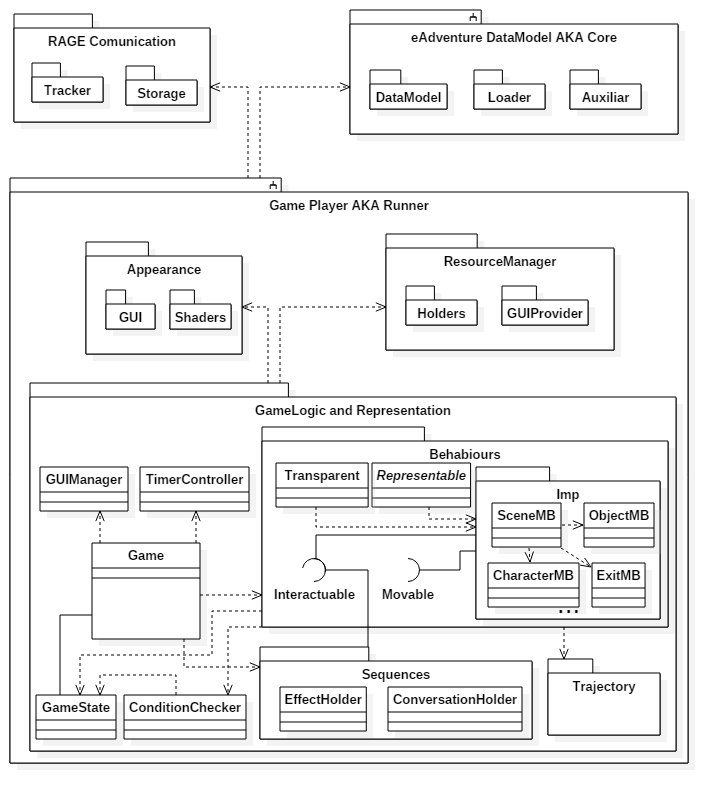
\includegraphics[height=6.3in]{figures/it2/Arquitectura.png}}
	\caption[Arquitectura - Versión Final]{Arquitectura del sistema, a nivel de paquetes de la versión final del proyecto}
	\label{arquitecturait2}
\end{figure}

\newpage

\subsection{El nucleo de Ejecución: Runner}

El núcleo de ejecución, también conocido como \textit{Runner}, está dividido en 3 subpaquetes, \textit{Apearance}, encargado de mejorar la representación visual, \textit{ResourceManager}, encargado de realizar la carga transparente de recursos, y \textit{GameLogic}, el cual podría considerarse el núcleo en si mismo, de lógica del juego. Estos tres paquetes surgen de la generalización de elementos que se encontraban, o bien en la antigua clase \textit{Game}, explicada en la sección \ref{gameit1}, o bien en alguna de las clases de utilidad, explicadas en la sección \ref{utilit1}.

De esta manera conseguimos que, la antigua clase controladora del juego \textit{Game}, y las Clases de Utilidad, ahora no tenga que realizar tantas tareas como realizaba anteriormente. En su lugar surgen 5 clases. Estas clases se encargan de hacer transparente la gestión de diversas tareas. Algunas de ellas realizan la gestión de un elemento en concreto, otras controlan la ejecución de otros elementos, y, por último otras se encargan de gestionar el estado del juego.

Estas 5 clases son:
\begin{enumerate}
	\item \textbf{Game}: La clase Game ha sido reducida para encargarse de tres tareas principales: En primer lugar, iniciar la carga y poner en funcionamiento el juego una vez esté cargado. En segundo lugar, controlar la interacción del usuario con los elementos del juego, ya sean elementos con representación, o elementos abstractos como secuencias. Y por último, ser la puerta de enlace que permite elegir qué escena se va a representar.
	
	\item \textbf{GUIManager}: Este gestor se encarga de realizar la gestión de la interfaz que antes se realizaba en \textit{Game}. Permite la emisión de burbujas de diálogo y el control sobre ellas, la posibilidad de mostrar una lista de opciones entre las que el usuario debe seleccionar una respuesta, y por último, la representación de acciones, como botones, y la gestión del menú contextual.
	
	\item \textbf{GameState}: Aunque \textit{GameState} no se considere un \textit{Manager} en si mismo, porque, a diferencia de todos los demás, no es un Singleton, siempre sigue habiendo una única Instancia, pues solo podemos tener un estado de juego, excepto cuando cargamos y guardamos partida. Maneja el estado del juego, que antes se realizaba en \textit{Game}, y facilita funciones para acceder a objetos de la especificación del juego, como \textit{Item} o \textit{NPC}.
	
	\item \textbf{TimerController}: Este gestor que se encarga de controlar los temporizadores que se utilizan en uAdventure para determinadas tareas, como, por ejemplo, hacer que un edificio se queme si no se ha evacuado a tiempo, es, tanto un \textit{Singleton}, como un \textit{MonoBehaviour}, pues necesita de la función \textit{Update()} para controlar que sus temporizadores no hayan saltado. Esta funcionalidad no estaba disponible en la anterior iteración.
	
	\item \textbf{ResourceManager}: este gestor se encarga de facilitar un repositorio transparente a través del cual acceder a los recursos del juego. Añade funcionalidades adicionales que no estaban disponibles anteriormente, como la persistencia en memoria de recursos para agilizar los tiempos de carga, la carga de vídeos, así como la carga de archivos de sonido.
\end{enumerate}

La representación de las clases que se explican en esta sección está disponible en la figura \ref{runnerbigit2}, junto a todas sus funciones. En este diagrama no están representados todos los elementos, pero si aquellos que han surgido de la evolución de las clases que se especificaron al comienzo de la sección. Este diagrama es bastante específico, pues contiene datos acerca de todas las funciones disponibles en cada uno de los elementos.

\begin{figure}[h]
	\centerline{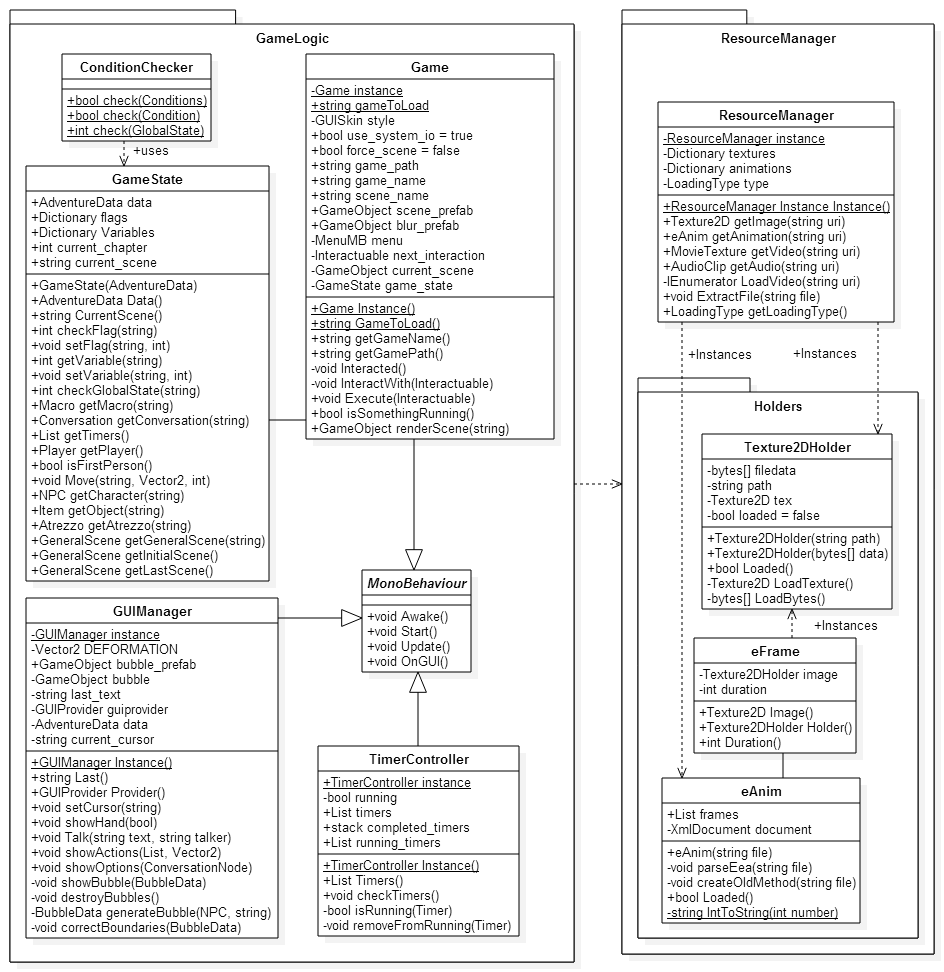
\includegraphics[height=7in]{figures/it2/GameLogicBigOnes.png}}
	\caption[GameLogic Grandes Gestores - Versión Final]{Diagrama de clases de los grandes gestores que controlan y proveen contenido para la ejecución del juego.}
	\label{runnerbigit2}
\end{figure}

\newpage


